\documentclass[/Users/ikedahajime/GitHub/reserch/master_report/thesis]{subfiles}
% このファイル内だけのコマンド
\begin{document}
\chapter{結果}
% \section{はじめに}
本章では計算結果および解析結果を述べる。
\secref{sec:result_abp}ではABPを、\secref{sec:result_cabp}ではCABPを
それぞれ壁の中に閉じ込めた時の結果について述べる。
\section{円に拘束されたABP}\label{sec:result_abp}
本節では、ABPを円形領域に閉じ込めた時の結果を示す。
\subsection{系全体のダイナミクス}
\subsubsection{低密度系}
本節では低密度系における系の流れについて論ずる。
%TODOずをみて論じる:図に使ったパラメータの説明
\begin{figure}
    \centering
    \begin{tabular}{c}
        \begin{minipage}{0.3\hsize}
            \text{(a)}
            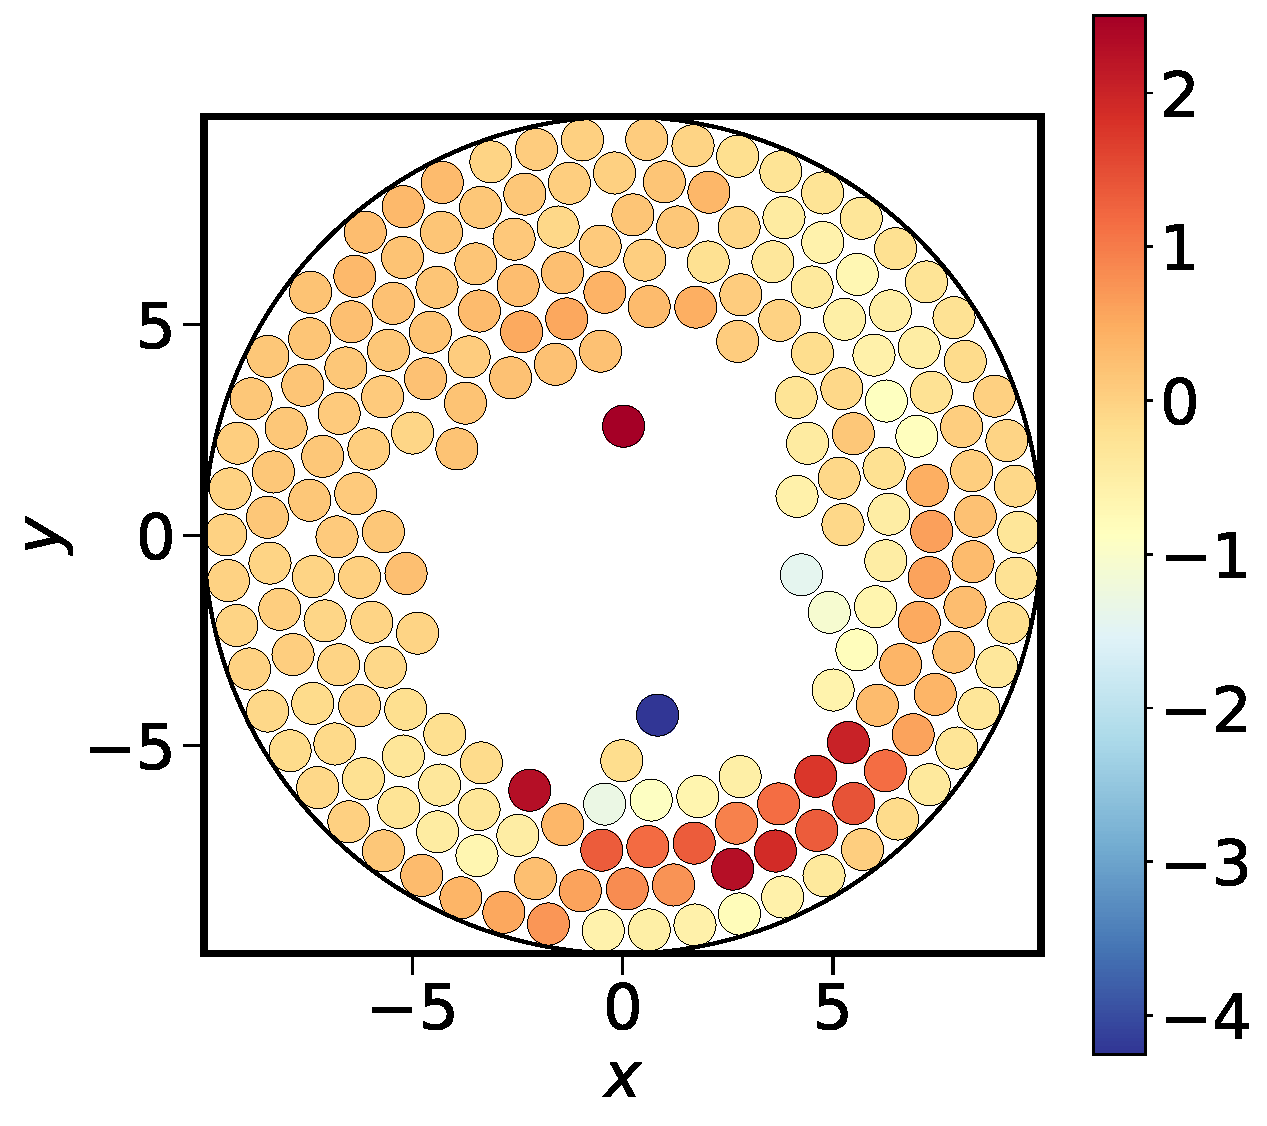
\includegraphics[width=\textwidth]{img/nabp/recap_mss_ani/arrR10_lo0.5_tau100.0_ms0.1.pdf}
        \end{minipage}\begin{minipage}{0.3\hsize}
            \text{(b)}
            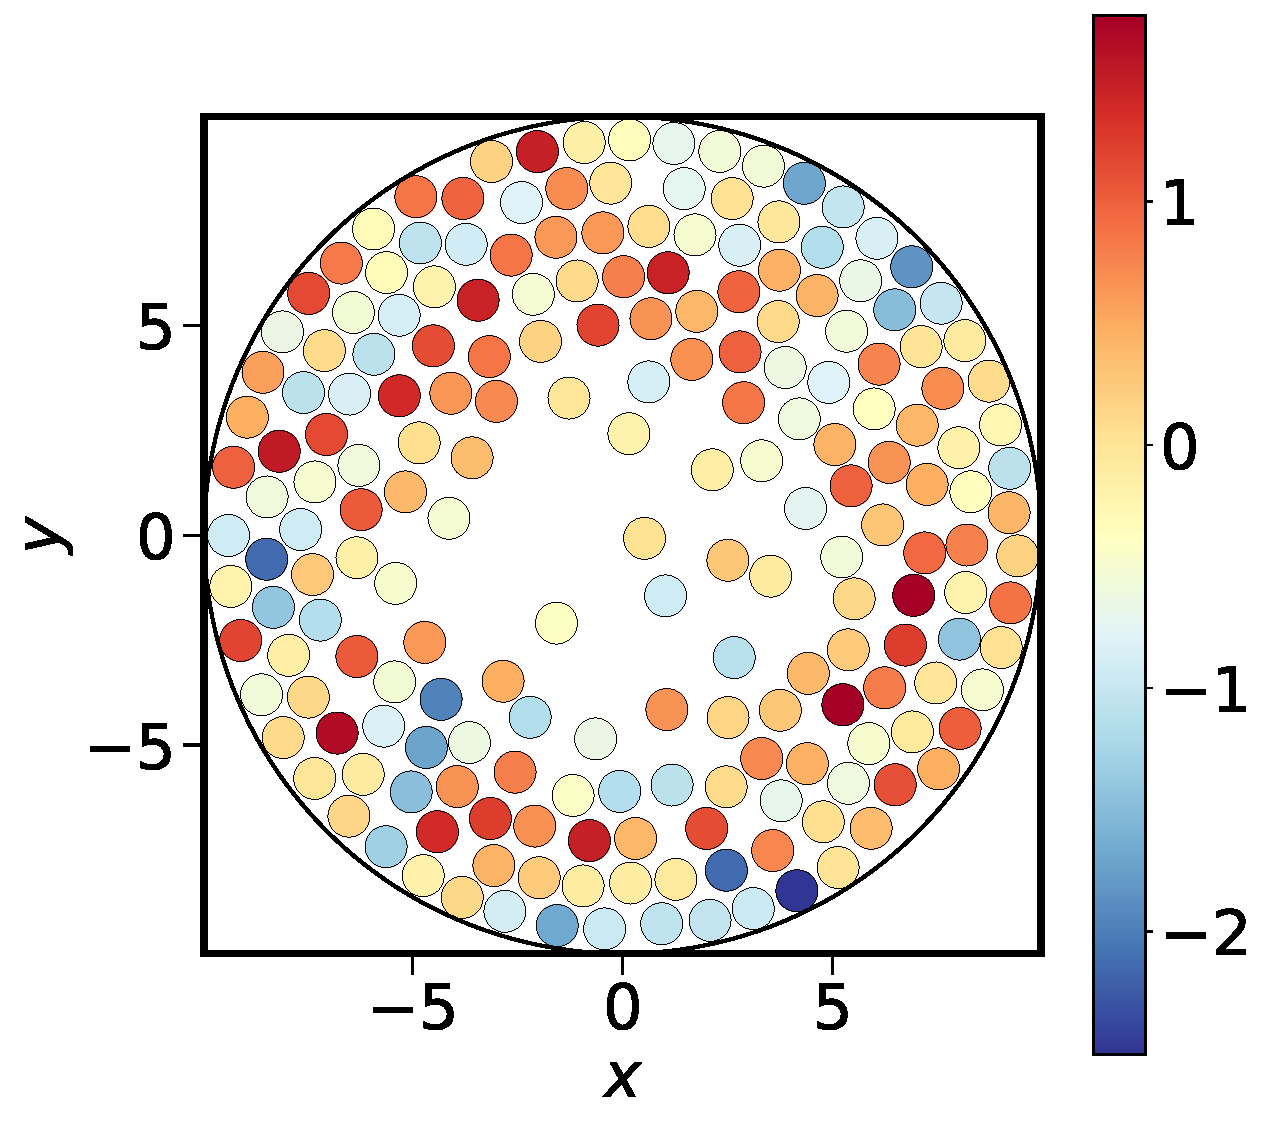
\includegraphics[width=\textwidth]{img/nabp/recap_mss_ani/arrR10_lo0.5_tau100.0_ms10.0.pdf}
        \end{minipage}
        \begin{minipage}{0.3\hsize}
            \text{(c)}
            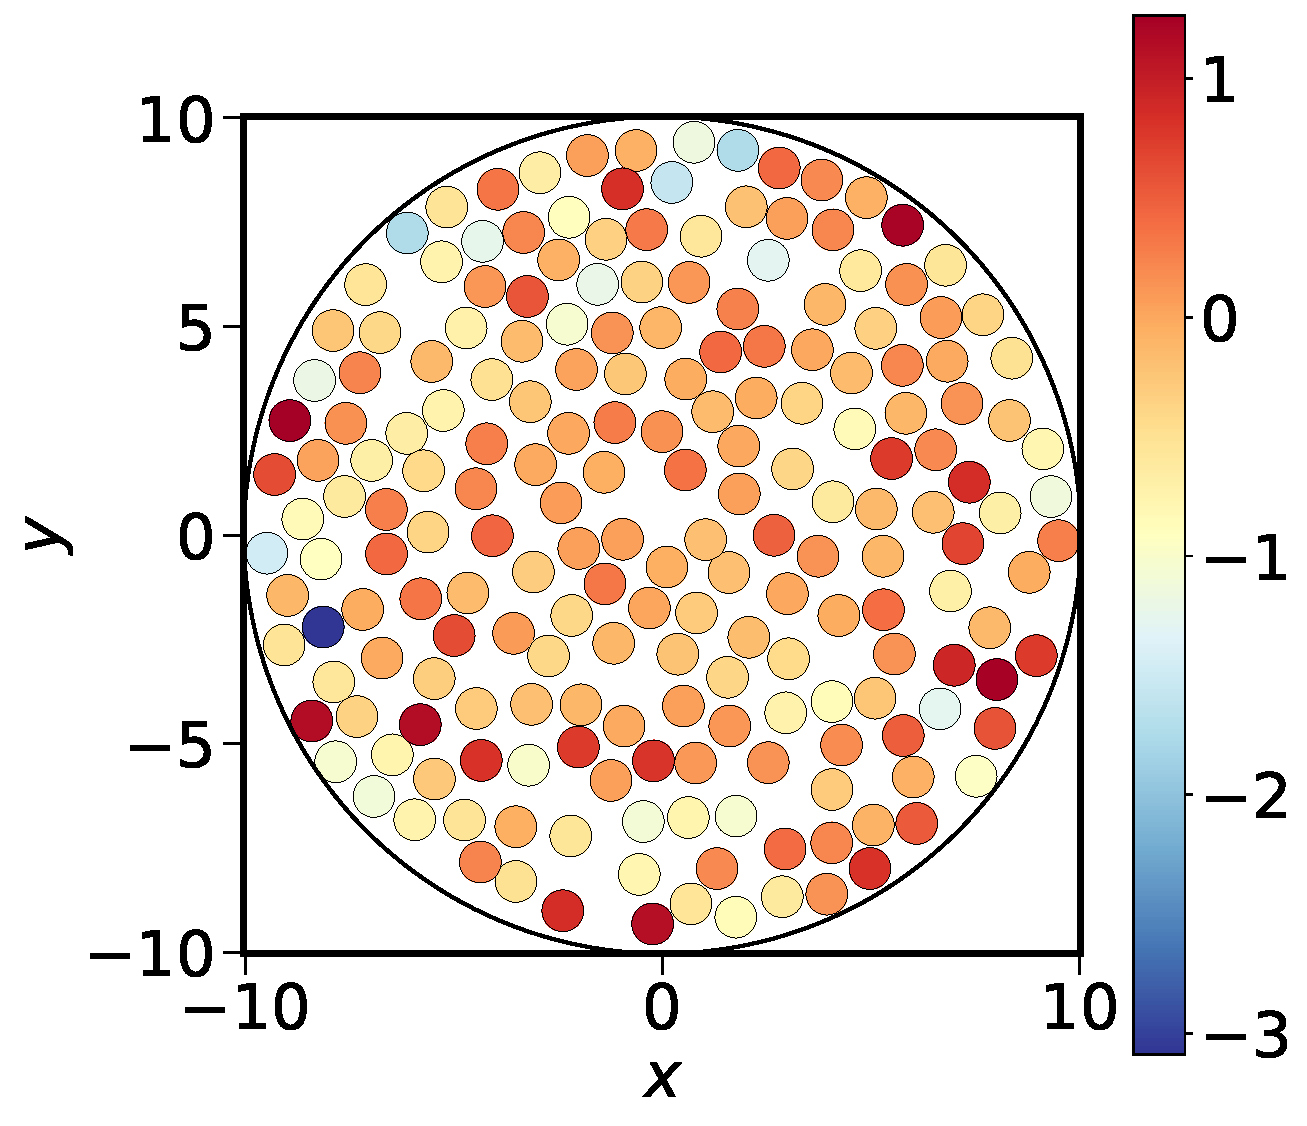
\includegraphics[width=\textwidth]{img/nabp/recap_mss_ani/arrR10_lo0.5_tau100.0_ms80.0.pdf}
        \end{minipage}

    \end{tabular}
    \caption[coor_lo]
    {
        $\varphi=0.5$における粒子配置。各図において、粒子の色は各粒子の角運動量を表す。
        パラメータは$Pe=100$を用い、(a) $M=0.1$ (b) $M=10$ (c) $M=100$ である。
    }
    \label{fig:nabp_coor_lodense}
\end{figure}
%fig:m=0.1
\figref{fig:nabp_coor_lodense}(a) を見ると、$M=0.1$の慣性が小さく$Pe$が大きな領域において粒子が壁に集まることがわかる。
これはABPを含むアクティブマター系においてよく見られる障害物への集積\cite{yangAggregationSegregationConfined2014}
と同様の現象であり、自己駆動誘起相分離 (Motility-Induced Phase Separation、略して MIPS)\cite{filyAthermalPhaseSeparation2012}
と同じ原理で発生していると考えられる。
この壁への集積は\figref{fig:nabp_coor_lodense}(b)、(c) のように
慣性の効果を大きくすることで抑制することができる。本研究ではMIPSによる影響を避けるため、
低密度系においては慣性が大きい領域について主に考える。


\figref{fig:nabp_lodense_psi_V}は、$\varphi=0.5、R=10$における、渦秩序変数$\psi$と規格化された角運動量$|V|$の
$Pe$および$M$依存性を表すグラフである。この図から、$M=10,80$
のいずれの系においても$\psi$の値は0.2を超えず、系は無秩序な運動をしていることが分かる。
\begin{figure}
    \centering
    \begin{tabular}{c}
        \begin{minipage}{0.4\hsize}
            \text{(a)}
            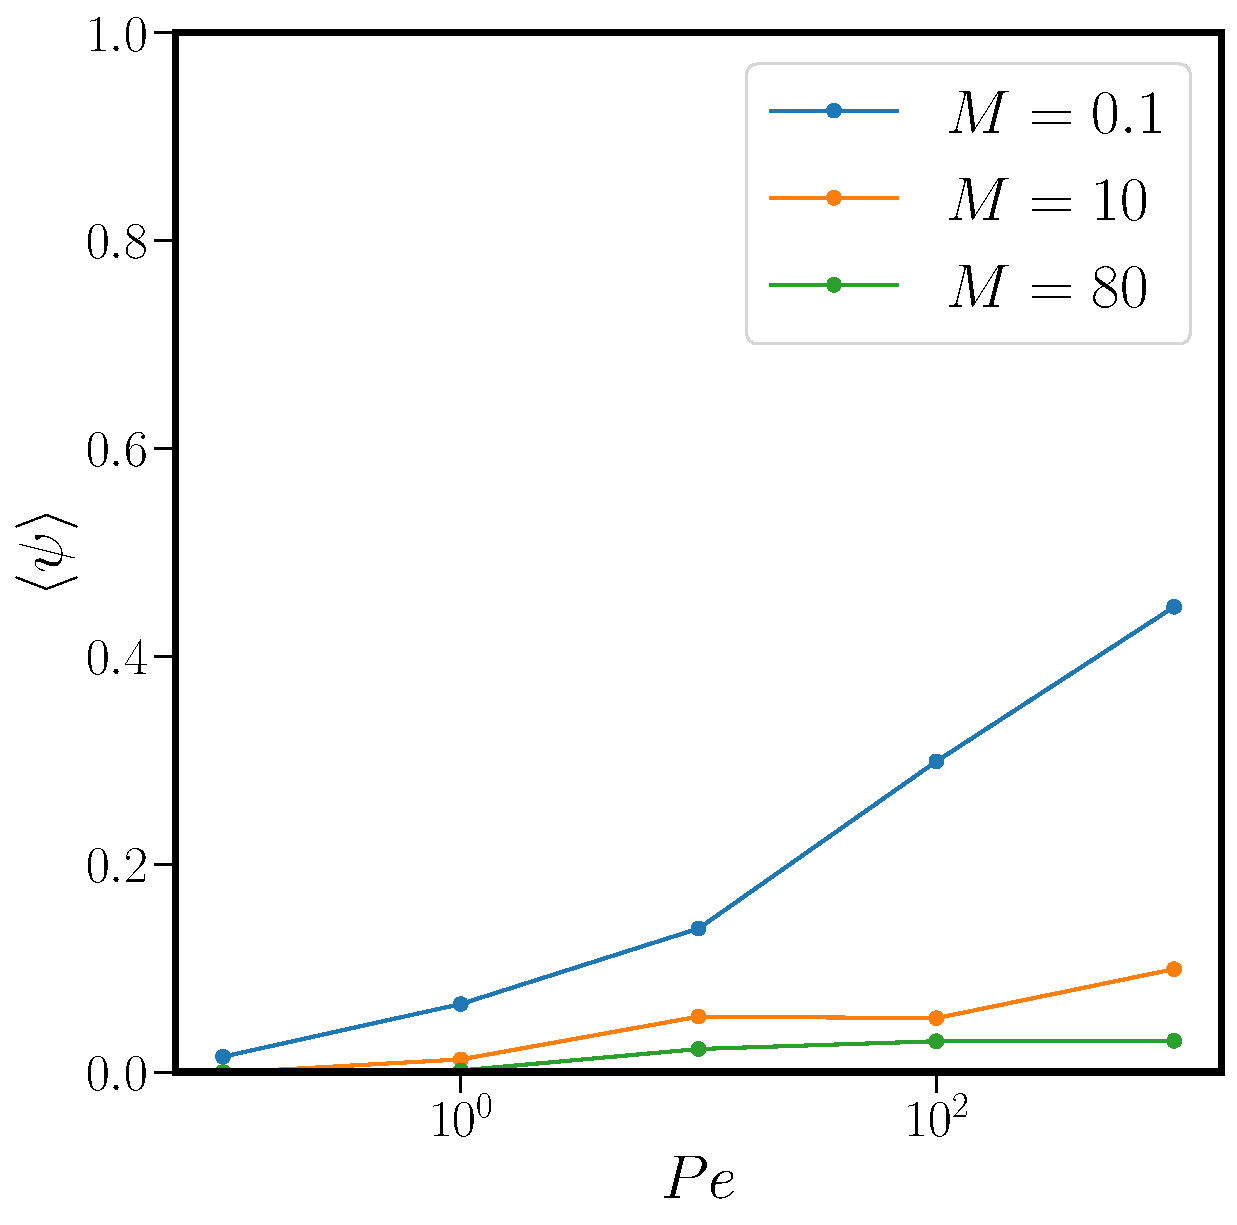
\includegraphics[width=\textwidth]{img/nabp/ens_r1/psi_0.5_[0.11080]_xsqFalse.pdf.pdf}
        \end{minipage}
        \begin{minipage}{0.4\hsize}
            \text{(b)}
            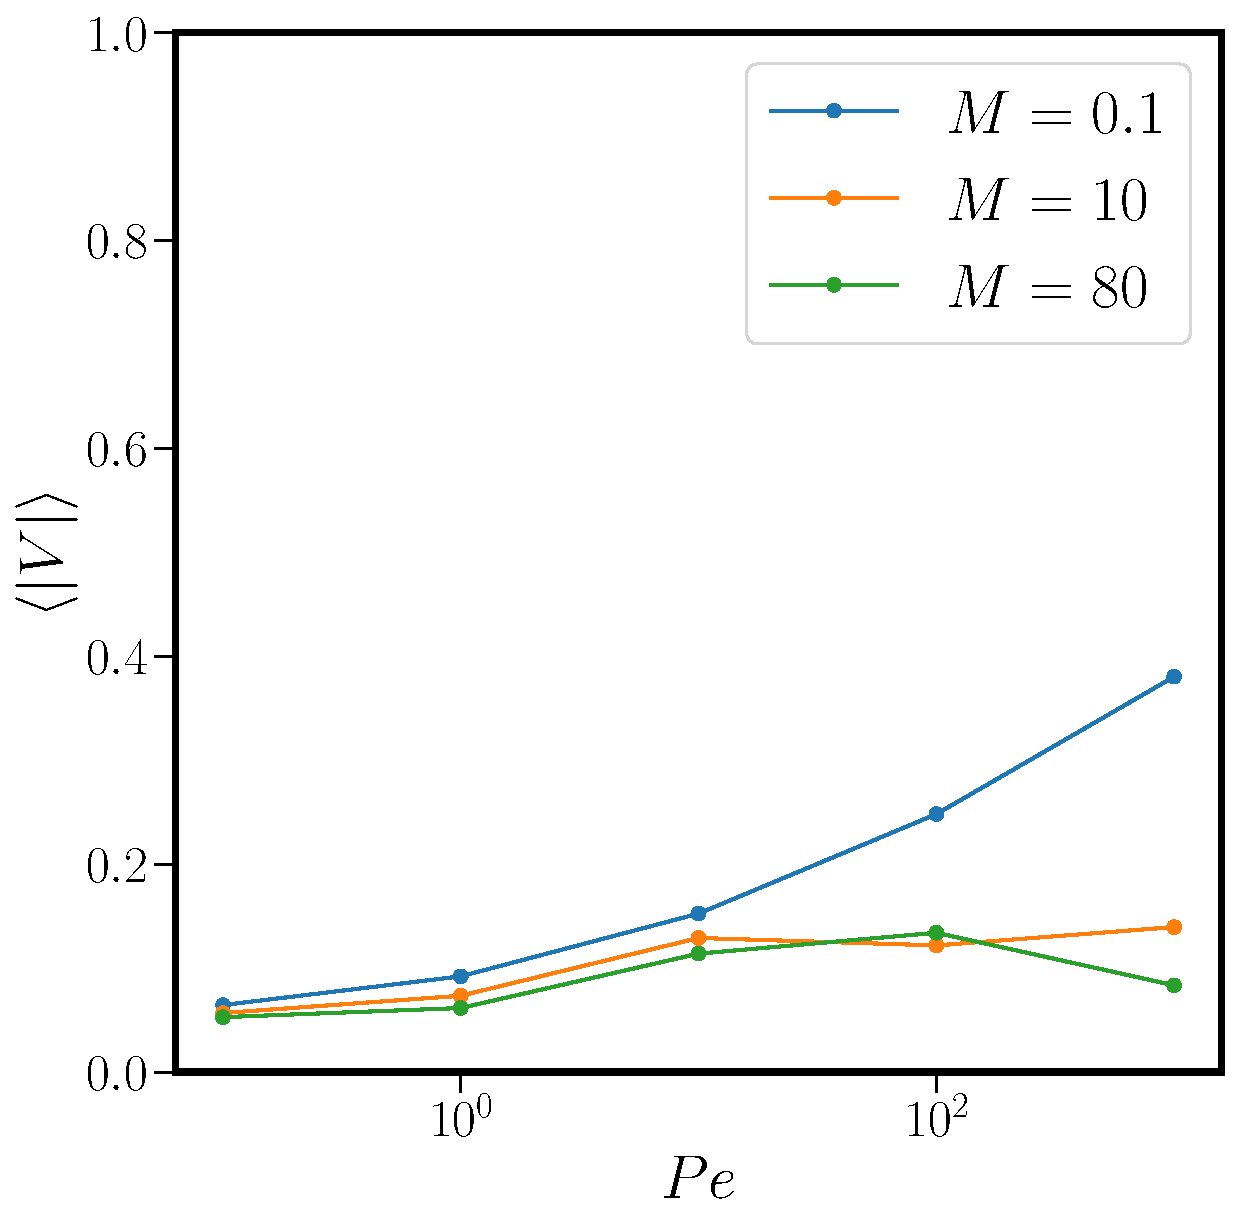
\includegraphics[width=\textwidth]{img/nabp/ens_r1/|V|_0.5_[0.11080]_xsqFalse.pdf}
        \end{minipage}
    \end{tabular}
    \caption[mdep_lodense]
    {
        $\varphi=0.5$におけるオーダーパラメータの$M$及び$Pe$依存性。
        (a) $\psi$ (b) $|V|$。系の半径$R=10$を選んだ。
    }
    \label{fig:nabp_lodense_psi_V}
\end{figure}

\subsubsection{高密度系}
続いて高密度系における系の流れについて見る。
\figref{fig:nabp_vabs_lo0.7_m}は、$\varphi=0.7、R=10$における、渦秩序変数$\psi$と規格化された角運動量$|V|$の
$Pe$および$M$依存性を表すグラフである。
まず$M$依存性について考えると、$\psi、|V|$のいずれのおいても
$M$が大きくなるにつれてパラメータの値が小さくなった。また各$M$における$Pe$依存性をみると、
定性的には変化しないことがわかる。よって、以降は$M=0.1$にのパラメータに注目して論じる。%考察?


\begin{figure}
    \centering
    \begin{tabular}{c}
        \begin{minipage}{0.4\hsize}
            \text{(a)}
            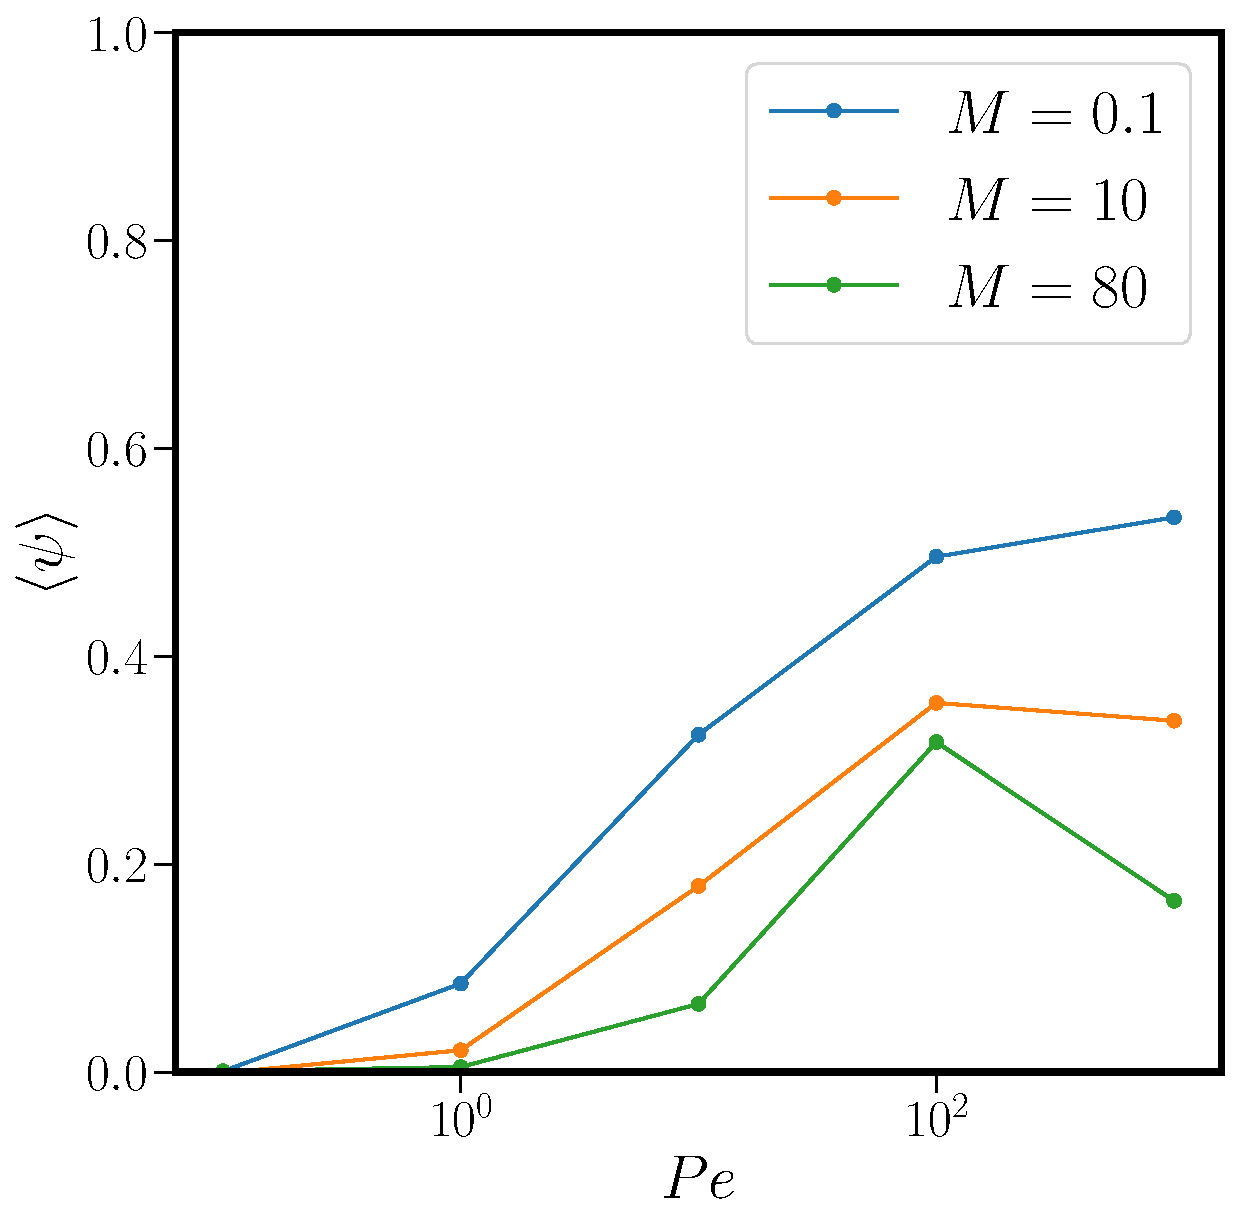
\includegraphics[width=\textwidth]{img/nabp/ens_r1/psi_0.7_[0.11080]_xsqFalse.pdf}
        \end{minipage}
        \begin{minipage}{0.4\hsize}
            \text{(b)}
            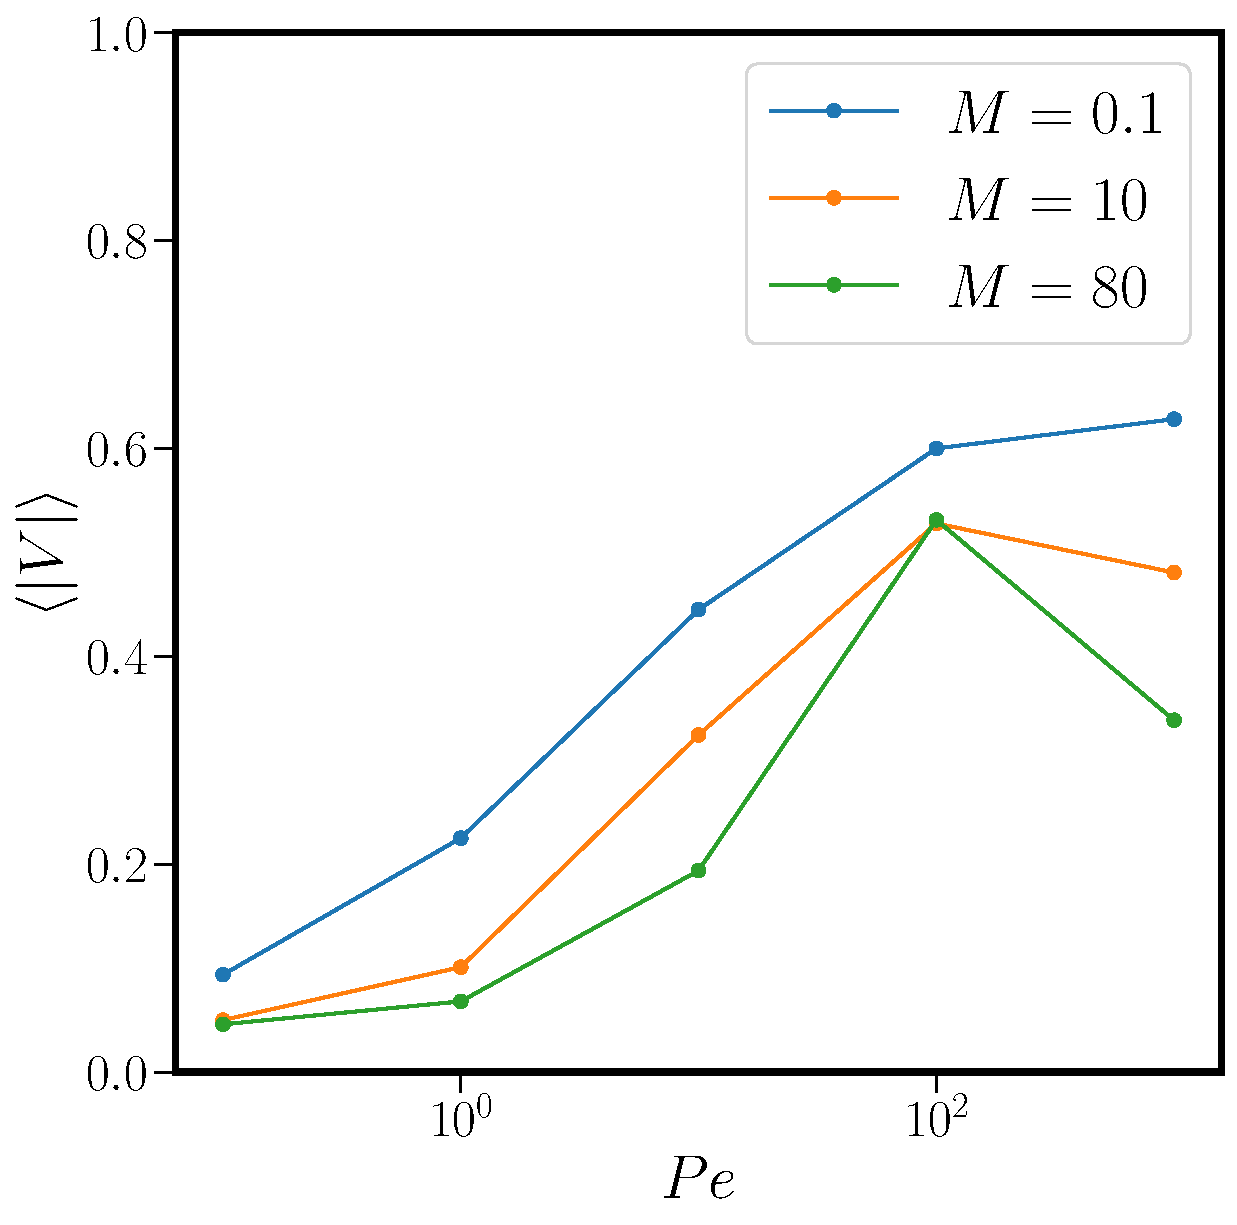
\includegraphics[width=\textwidth]{img/nabp/ens_r1/|V|_0.7_[0.11080]_xsqFalse.pdf.pdf}
        \end{minipage}
    \end{tabular}
    \caption[Four sample images]
    {
        $\varphi=0.7$におけるオーダーパラメータの$M$及び$Pe$依存性。
        (a) $\psi$ (b) $|V|$。系の半径$R=10$を選んだ。
    }
    \label{fig:nabp_vabs_lo0.7_m}
\end{figure}
次に$Pe$依存性に注目する。図から、$Pe$が大きくなると$\psi$及び$|V|$の値が大きくなる、
つまり粒子が同じ方向へと流れることがわかる。これは先行研究\cite{capriniCollectiveEffectsConfined2021}
におけるオーダーパラメータの変化と定性的に同じであり、同様のメカニズム
で変化していると考えられる。しかし$|V|$の絶対値は最大でも0.6であり、
先行研究\cite{capriniCollectiveEffectsConfined2021}より小さい値、つまり流れが先行研究に比べて
発生した流れが安定していないことを示す。

\subsection{時間依存性}
% 生の時間依存(図)は、高密度系における$V(t)$を時間の関数としてプロットした図である。
% この図を見ると、$Pe$が大きな領域において、一見規則正しく周期的に運動しているように見える。
この時間依存性を定量的に評価するため、時間についてフーリエ変換を行った。
その結果が\figref{fig:fourie_transform}(a)である。
この図は密度$\varphi=0.7、M=0.1$における全角運動量のフーリエ変換のスペクトルである。
この図から、$Pe$が1より大きい領域では周波数$\omega$が大きな領域において、そのスペクトルが
$\omega^{-2}$に比例していることがわかる。これは一粒子状態のABPにおける速度相関のスペクトル
と一致する。実際に、$C(\omega)=C_0/(1+(\tau_{corr}\omega)^2)$でフィッティングした時の
$\tau_{corr}$と Péclet 数$Pe$の関係をプロットした図(\figref{fig:fourie_transform}(b))
を見ると分かる。%TODO::taucorrに名前づけ
この図から、$\tau_{corr}$が$ Pe$に比例することが分かる。これは一粒子状態のABPにおける速度相関のスペクトル%TODO:指揮をかく
と同様であり、これはこの系における系全体の回転の時間依存性は一粒子描像で描けることを示している。

\begin{figure}
    \centering
    \begin{tabular}{c}
        \begin{minipage}{0.4\hsize}
            \text{(a)}
            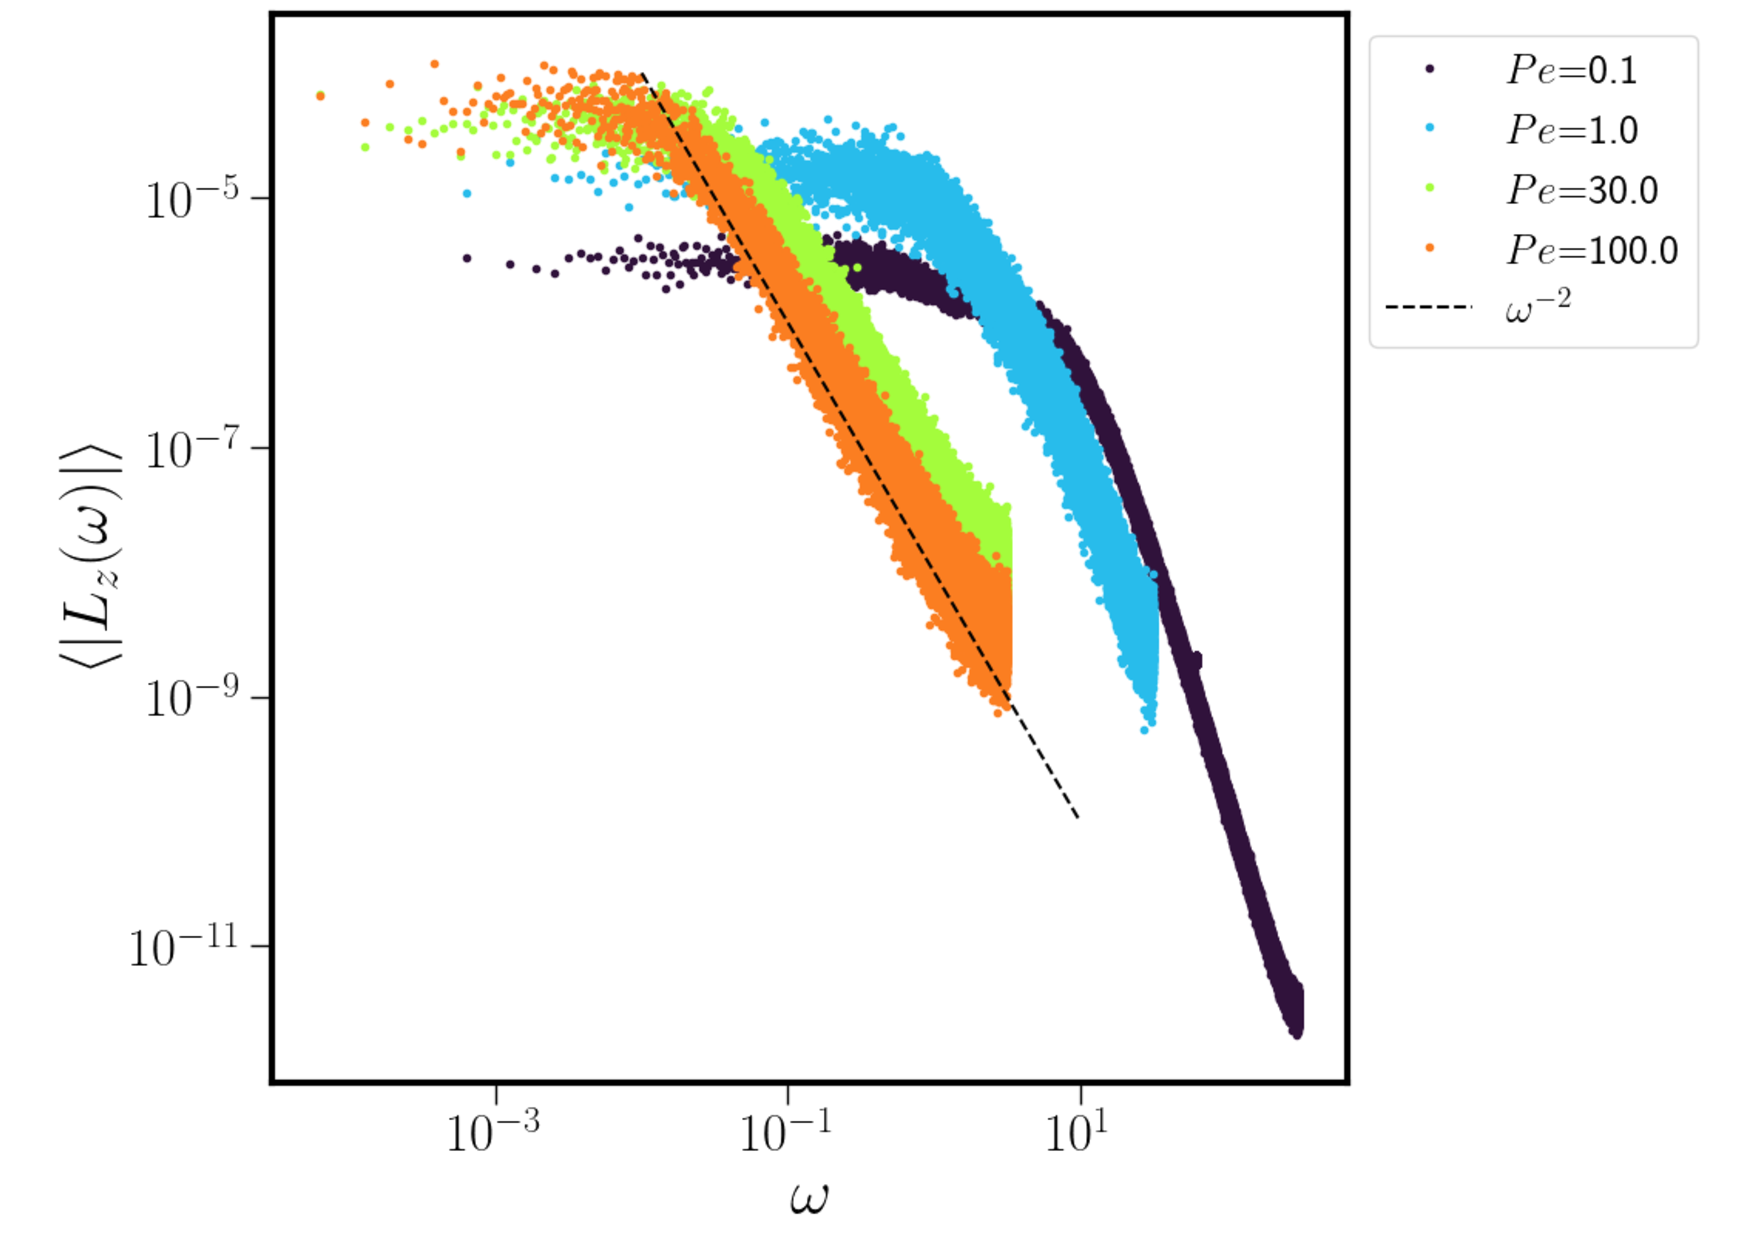
\includegraphics[width=\textwidth]{img/nabp/ens_r1/ft_lzlo0.7Ms0.1tMg0R10Rbit0.0v021.pdf}
        \end{minipage}
        \begin{minipage}{0.4\hsize}
            \text{(b)}
            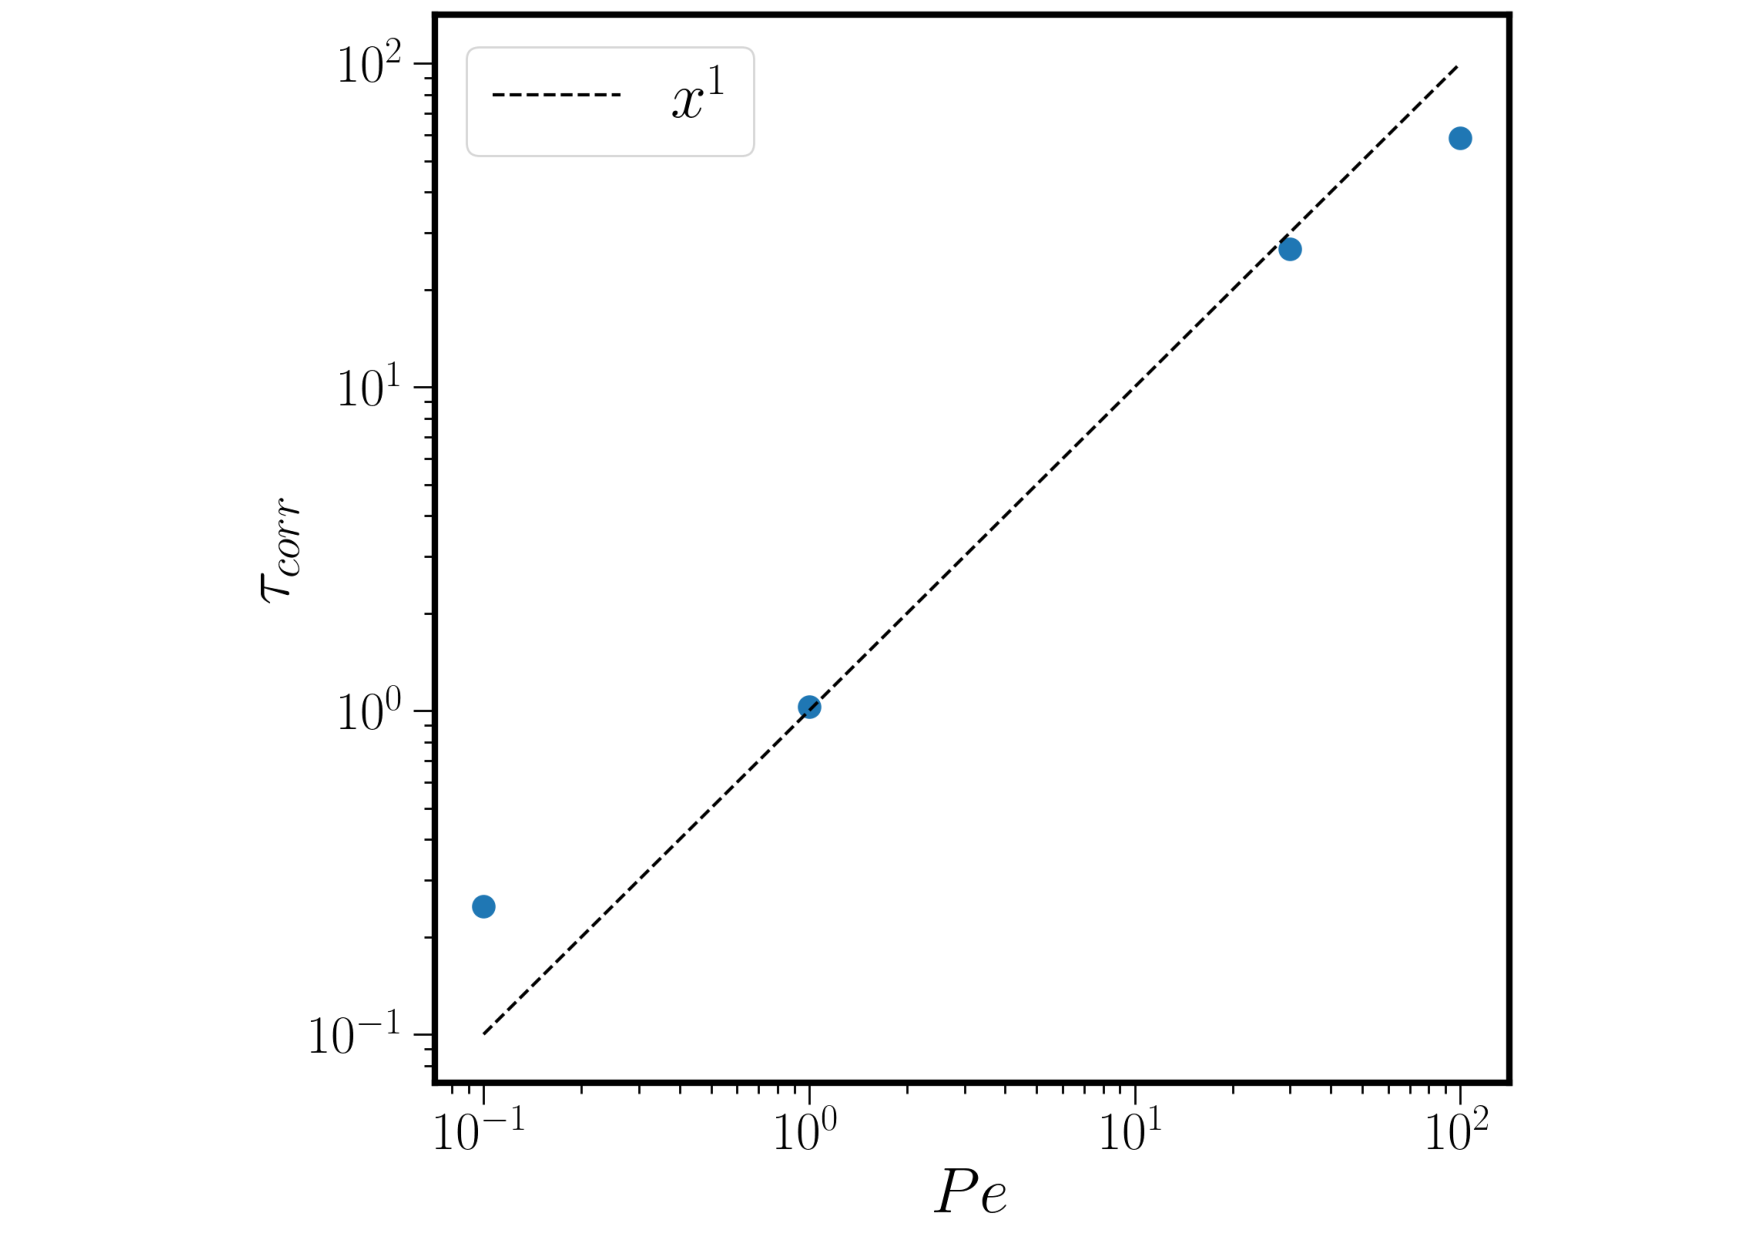
\includegraphics[width=\textwidth]{img/nabp/ens_r1/ft_taucorr_lo0.7_m0.1.pdf}
        \end{minipage}
    \end{tabular}
    \caption[fourie_transform]
    {
        (a) $\varphi=0.7、M=0.1$ における$L_z$の時間についてのフーリエ変換。図中の点線は$\omega^{-2}$を表す。
        (b) $C_0/(1+(\tau_{corr}\omega)^2)$でフィッティングした時の$\tau_{coor}$対$Pe$のグラフ
    }
    \label{fig:fourie_transform}
\end{figure}
また、\figref{fig:fourie_transform}(a)を見ると、$Pe=0.1$の時周波数$\omega$が大きな
領域で$\omega^{-4}$に比例している。これは$M=0.1$の系でシミュレーションを行なっており、
$M\simeq\tau$のため、慣性による緩和時間と自己駆動力による
緩和時間が等しいため起きていると考えられる。
\end{document}
